\section{Resultados}

\subsection{An\'alisis Exploratorio del Dataset}
El dataset Iris presenta una estructura donde la clase setosa es linealmente separable. Las clases versicolor y virginica presentan solapamiento parcial, particularmente en las dimensiones de s\'epalo (Figura~\ref{fig:eda}).

\begin{figure*}[t]
\centering
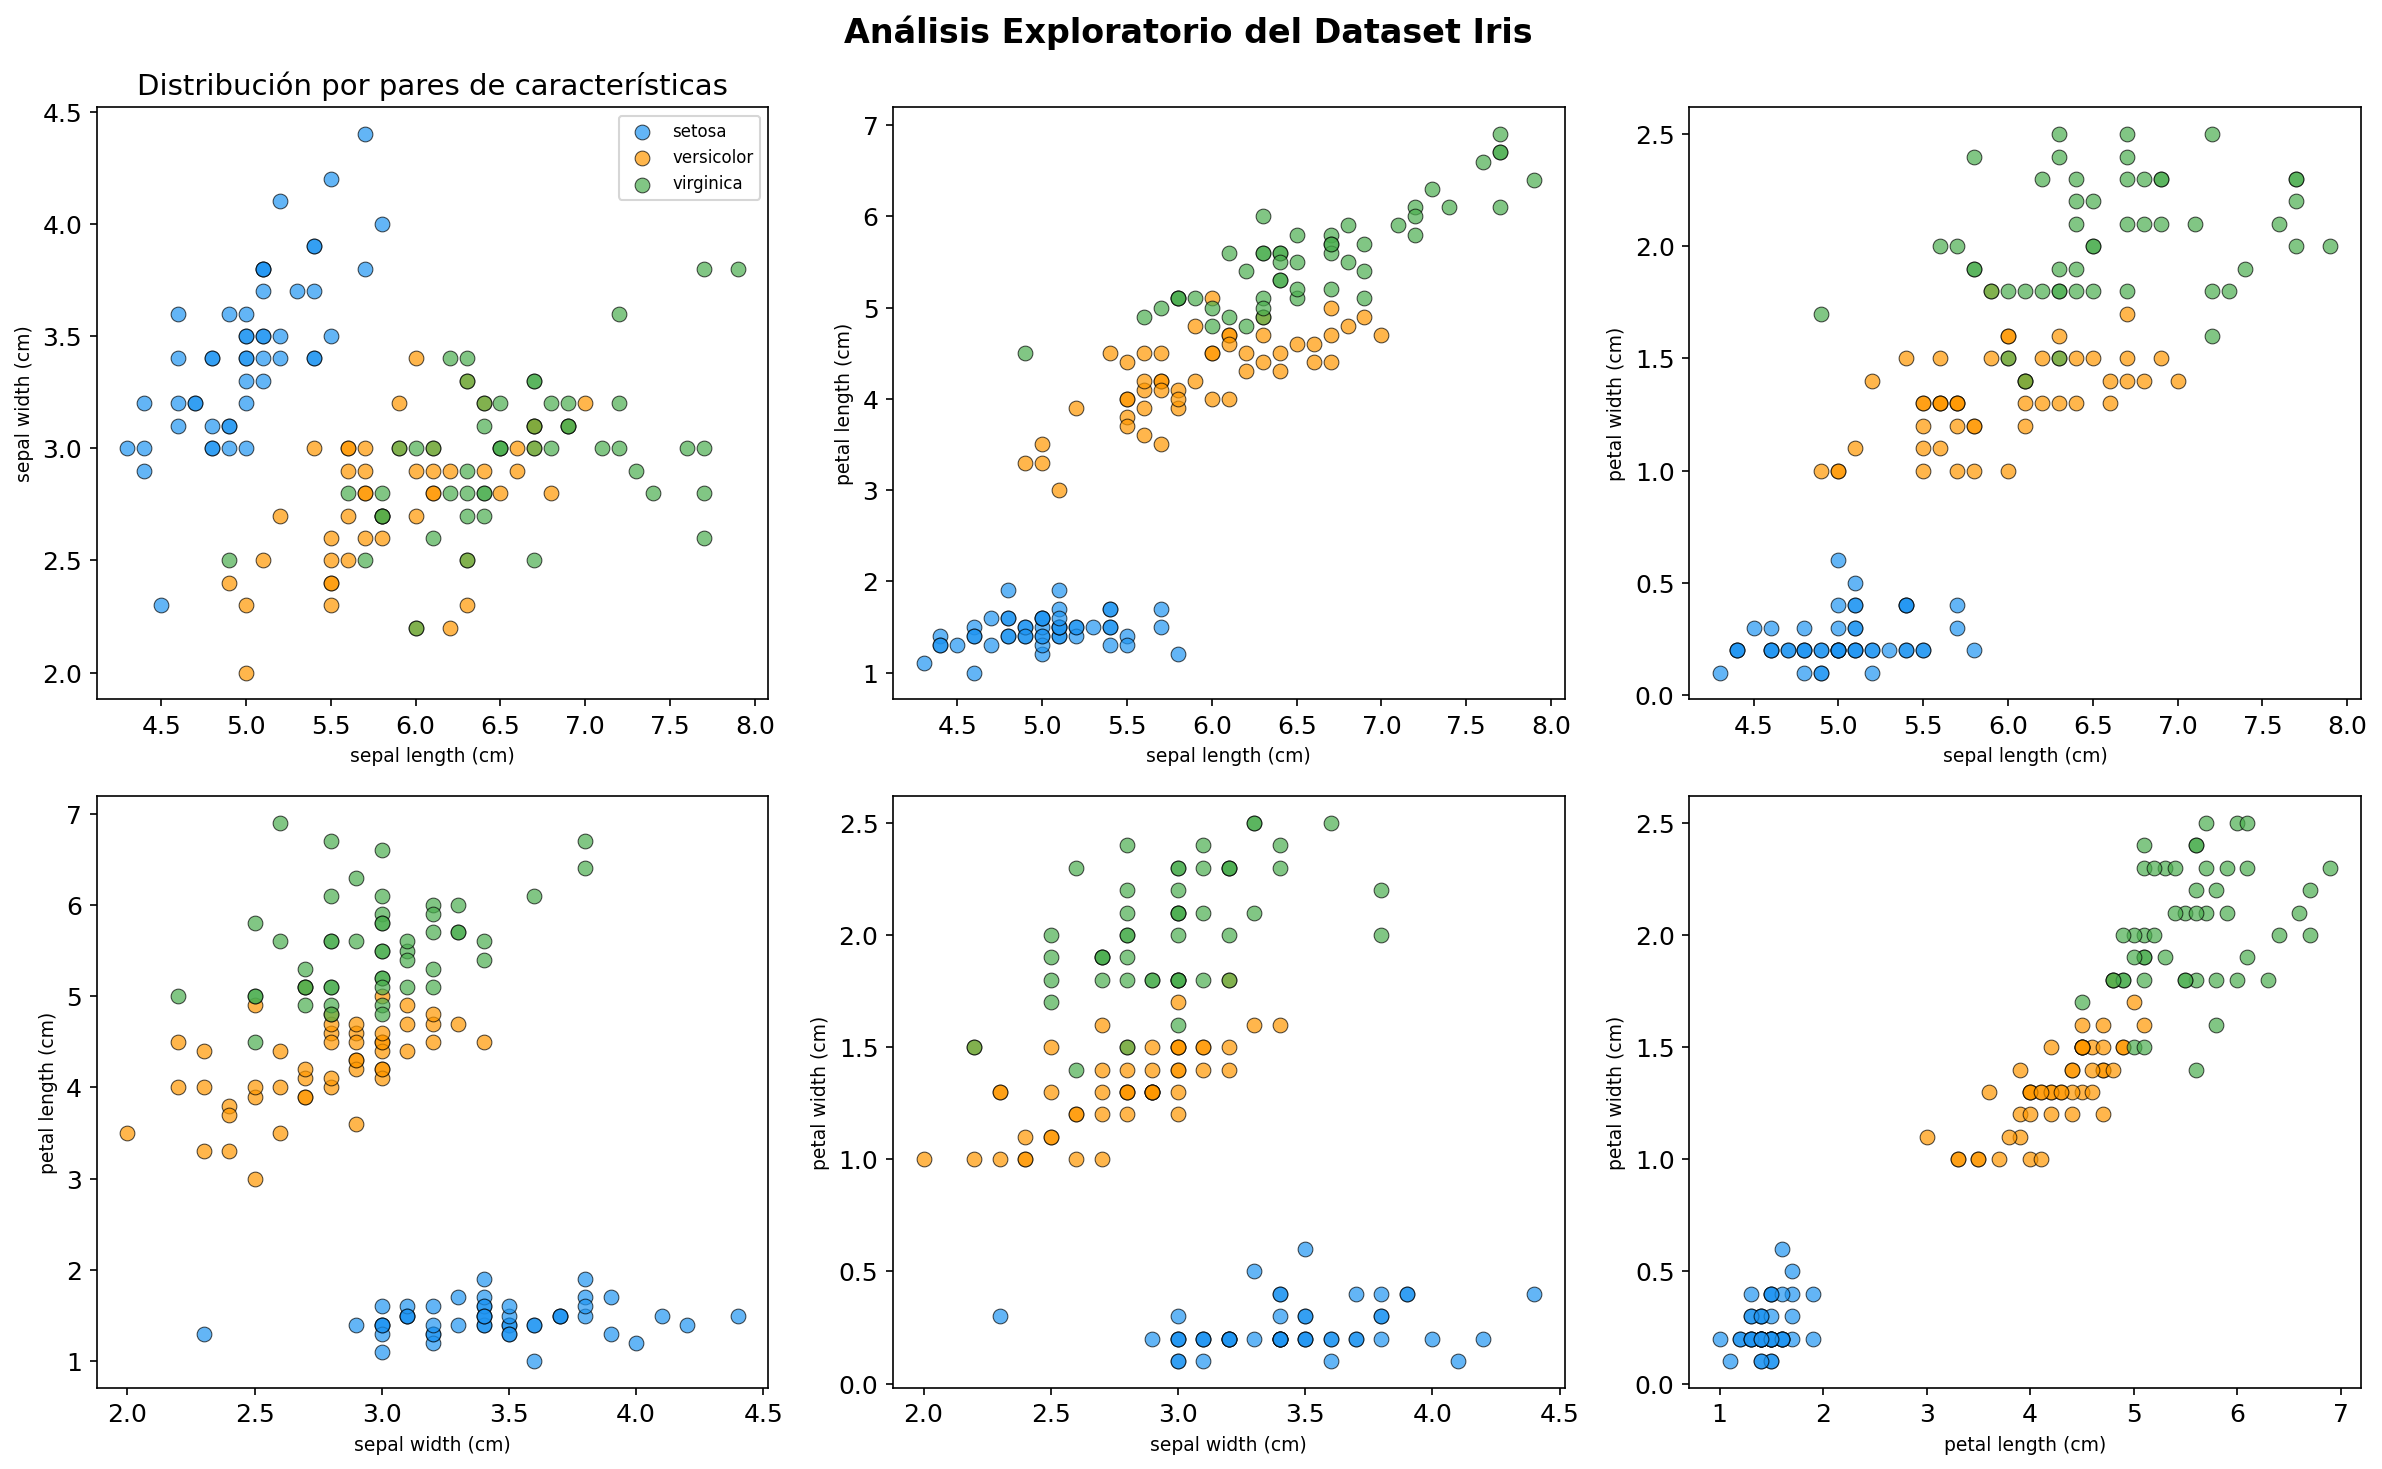
\includegraphics[width=0.92\textwidth]{figuras/eda_iris.png}
\caption{Distribuci\'on de las muestras de Iris por pares de caracter\'isticas. Setosa (azul) es claramente separable de versicolor y virginica.}
\label{fig:eda}
\end{figure*}

\subsection{Resultados de Modelos Cl\'asicos}
Los tres modelos cl\'asicos alcanzaron un accuracy de 93.33\% en el conjunto de test (Tabla~\ref{tab:clasicos}). La validaci\'on cruzada 5-fold confirm\'o la estabilidad de estos resultados.

\begin{table}[H]
\centering
\caption{Resultados de modelos cl\'asicos en Iris}
\label{tab:clasicos}
\small
\begin{tabular}{lcccc}
\toprule
\textbf{Modelo} & \textbf{Acc.} & \textbf{Prec.} & \textbf{F1} & \textbf{T (s)} \\
\midrule
SVM-RBF & 0.933 & 0.935 & 0.933 & 0.001 \\
MLP     & 0.933 & 0.935 & 0.933 & 0.108 \\
KNN     & 0.933 & 0.944 & 0.933 & $<$0.001 \\
\bottomrule
\end{tabular}
\end{table}

\subsection{Resultados de Modelos Cu\'anticos}

\subsubsection{VQC}
El VQC alcanz\'o un accuracy de 37.78\% en 200 iteraciones de COBYLA, con un tiempo de 34.3s. La curva de convergencia (Figura~\ref{fig:vqc_loss}) muestra que la funci\'on de p\'erdida no convergi\'o completamente, consistente con la dificultad de optimizar circuitos variacionales en problemas multiclase.

\begin{figure}[H]
\centering
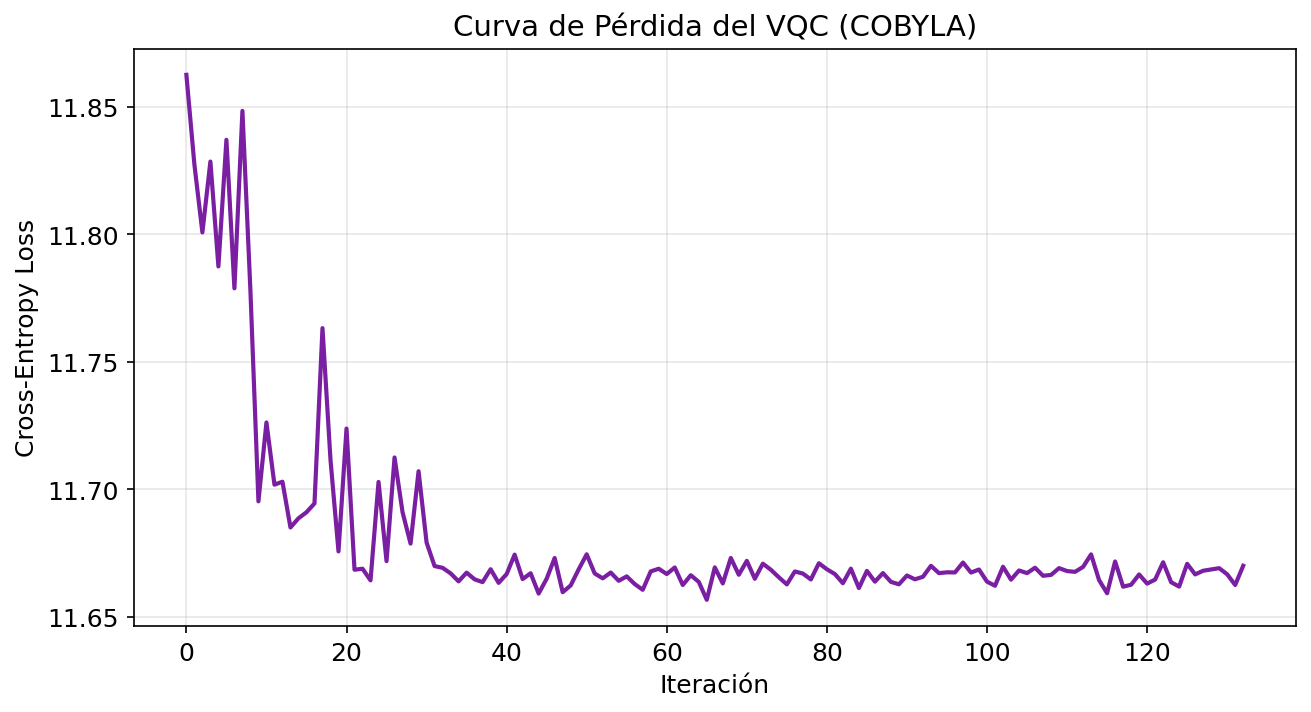
\includegraphics[width=\columnwidth]{figuras/vqc_loss.png}
\caption{Evoluci\'on de la entrop\'ia cruzada durante el entrenamiento del VQC con COBYLA (200 iteraciones).}
\label{fig:vqc_loss}
\end{figure}

\subsubsection{QSVC}
El QSVC obtuvo un accuracy de 77.78\% con un tiempo de 10.6s. Su rendimiento superior al VQC se debe a que el kernel cu\'antico opera en el espacio de Hilbert completo sin requerir optimizaci\'on variacional.

\subsection{Comparaci\'on General}
La Tabla~\ref{tab:comparacion} y la Figura~\ref{fig:comparacion} resumen la comparaci\'on entre todos los modelos.

\begin{table}[H]
\centering
\caption{Comparaci\'on de todos los modelos en Iris}
\label{tab:comparacion}
\small
\begin{tabular}{llccc}
\toprule
\textbf{Modelo} & \textbf{Tipo} & \textbf{Acc.} & \textbf{F1} & \textbf{T (s)} \\
\midrule
SVM-RBF & Cl\'as. & 0.933 & 0.933 & 0.001 \\
MLP     & Cl\'as. & 0.933 & 0.933 & 0.108 \\
KNN     & Cl\'as. & 0.933 & 0.933 & $<$0.001 \\
VQC     & Cu\'ant. & 0.378 & 0.338 & 34.27 \\
QSVC    & Cu\'ant. & 0.778 & 0.777 & 10.63 \\
\bottomrule
\end{tabular}
\end{table}

\begin{figure*}[t]
\centering
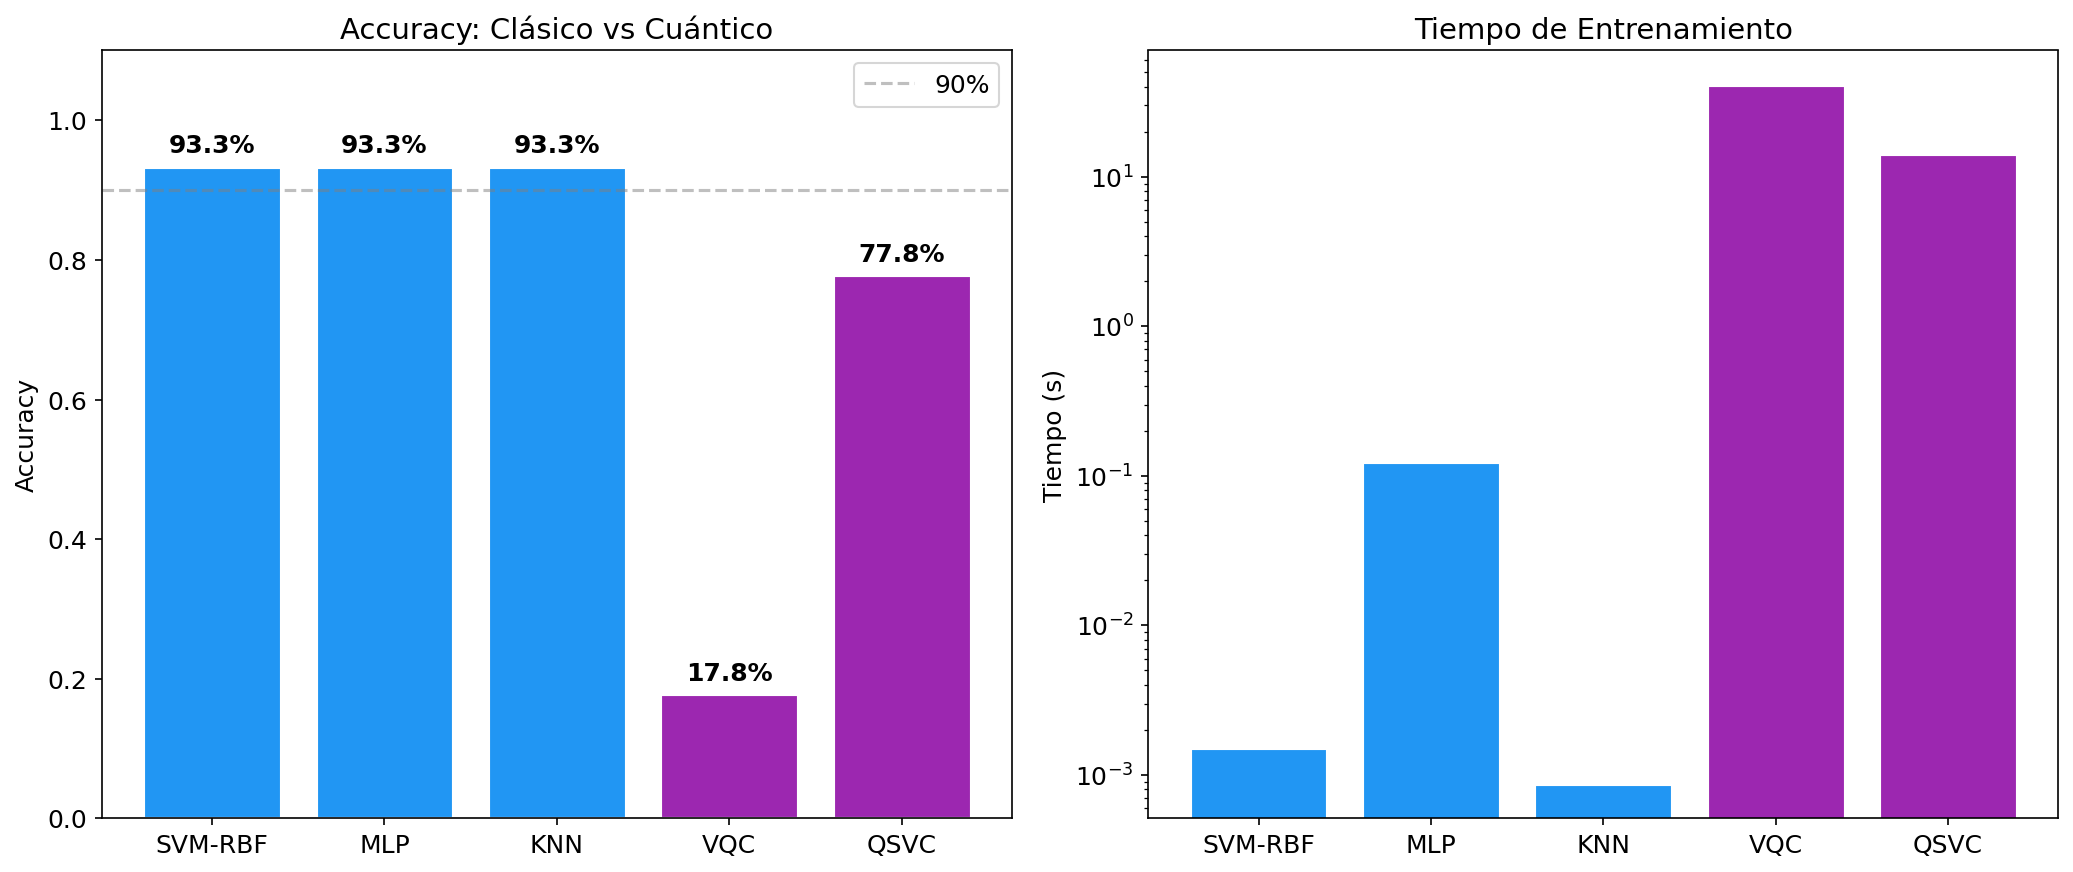
\includegraphics[width=0.92\textwidth]{figuras/comparacion_general.png}
\caption{Izquierda: accuracy por modelo. Derecha: tiempo de entrenamiento (escala logar\'itmica). Azul = cl\'asico, morado = cu\'antico.}
\label{fig:comparacion}
\end{figure*}

\subsection{Matrices de Confusi\'on}
La Figura~\ref{fig:confusion} muestra las matrices de confusi\'on. El VQC tiene dificultades para distinguir entre las tres clases, mientras que QSVC confunde principalmente versicolor con virginica.

\begin{figure*}[t]
\centering
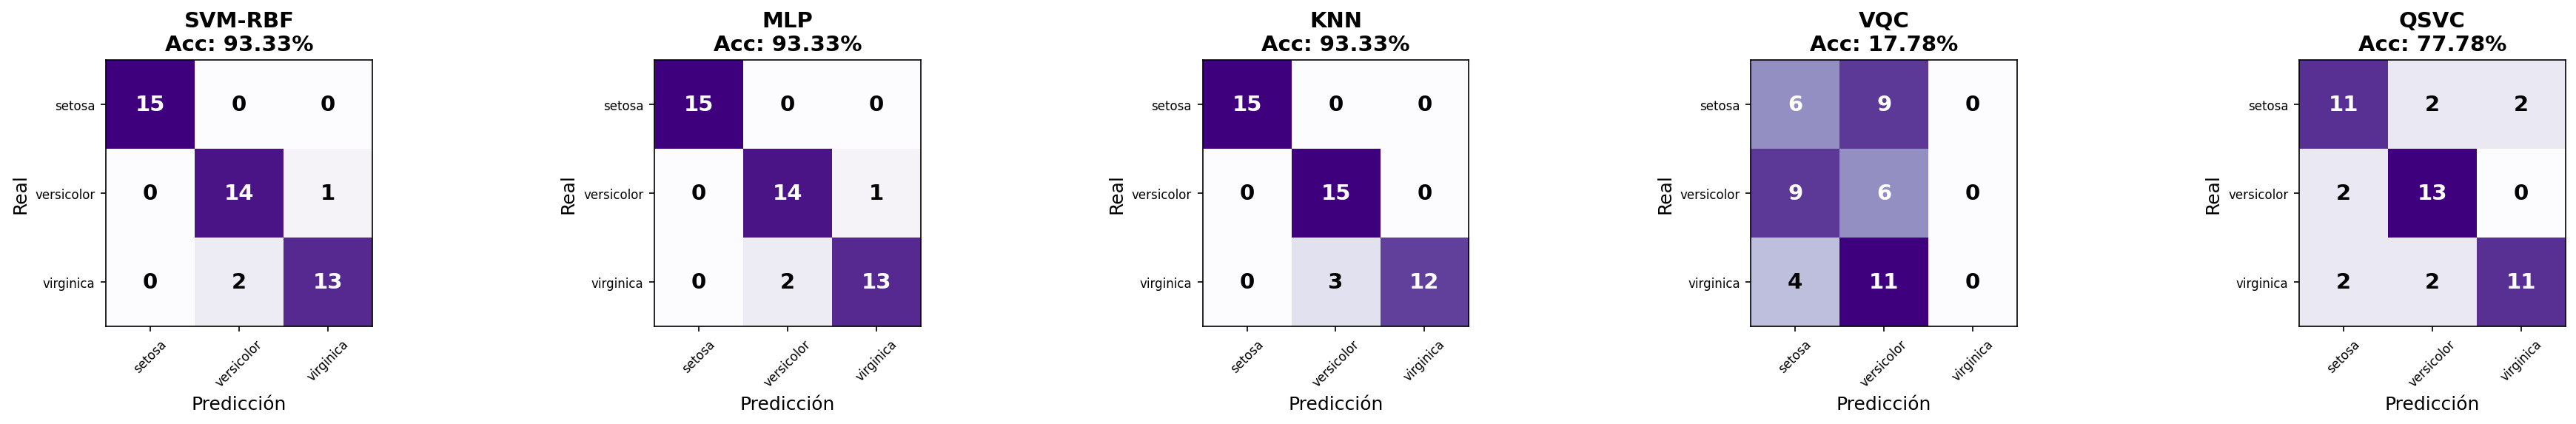
\includegraphics[width=0.92\textwidth]{figuras/matrices_confusion.png}
\caption{Matrices de confusi\'on para los cinco modelos evaluados sobre el conjunto de test de Iris.}
\label{fig:confusion}
\end{figure*}

\subsection{Fronteras de Decisi\'on}
La Figura~\ref{fig:frontera} muestra la frontera de decisi\'on del SVM-RBF en una proyecci\'on PCA bidimensional, donde se aprecian las regiones de clasificaci\'on no lineales.

\begin{figure}[H]
\centering
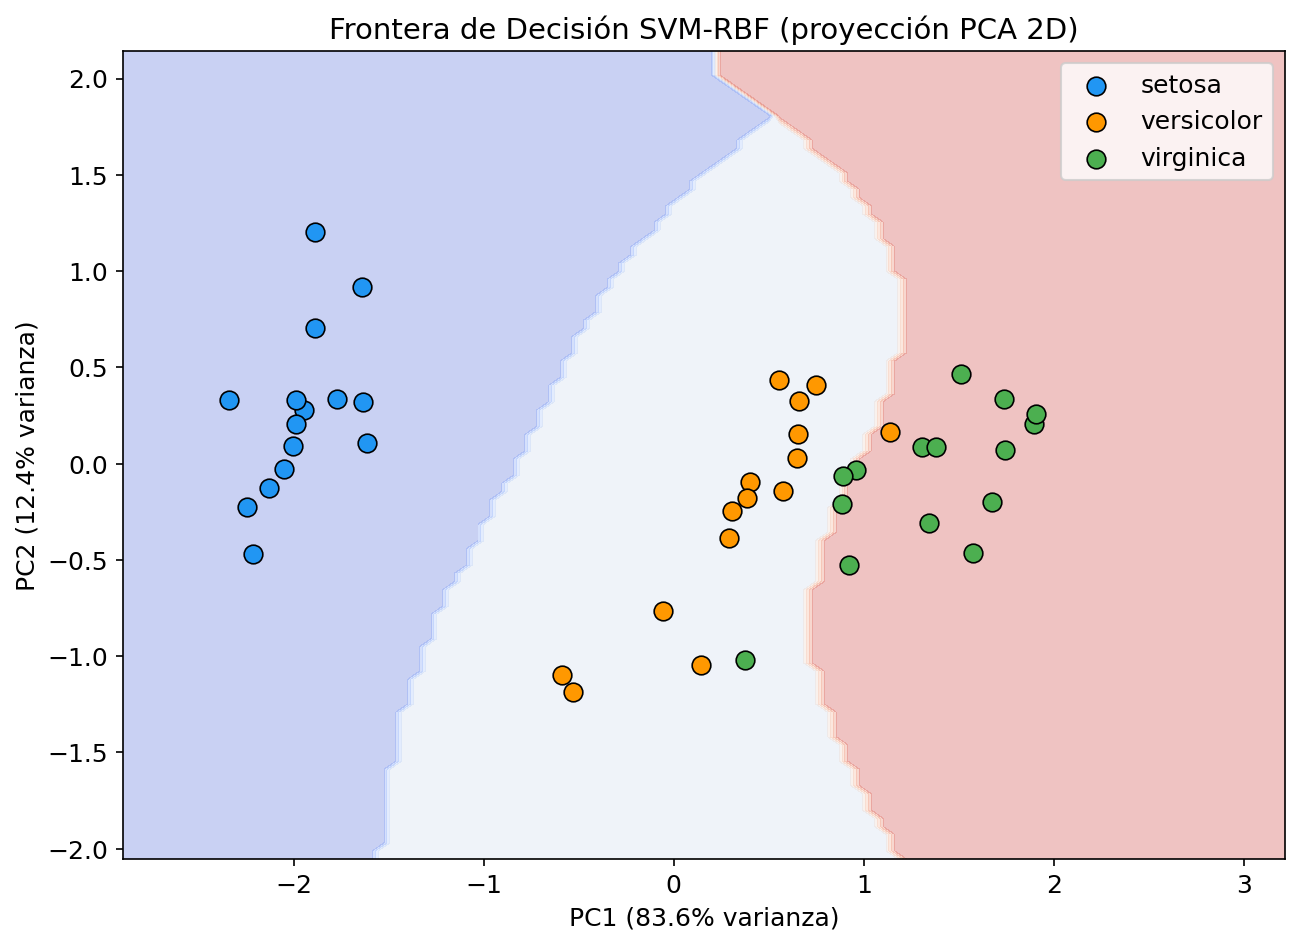
\includegraphics[width=\columnwidth]{figuras/frontera_decision.png}
\caption{Frontera de decisi\'on del SVM-RBF proyectada en las dos primeras componentes principales (PCA 2D).}
\label{fig:frontera}
\end{figure}

\subsection{Exp. 1: Comparaci\'on de Feature Maps}
Se evaluaron cuatro feature maps manteniendo fijo el ansatz (RealAmplitudes, reps=3). Los resultados (Tabla~\ref{tab:featuremaps}) muestran que ZFeatureMap obtuvo el mejor accuracy (66.67\%) a pesar de su menor profundidad.

\begin{table}[H]
\centering
\caption{Comparaci\'on de feature maps}
\label{tab:featuremaps}
\small
\begin{tabular}{lccc}
\toprule
\textbf{Feature Map} & \textbf{Acc.} & \textbf{Prof.} & \textbf{T (s)} \\
\midrule
ZFeatureMap       & 0.667 & 15 & 34.6 \\
ZZFeatMap (lin.)  & 0.578 & 29 & 40.1 \\
ZZFeatMap (full)  & 0.489 & 41 & 52.7 \\
PauliFeatureMap   & 0.556 & 41 & 61.8 \\
\bottomrule
\end{tabular}
\end{table}

\begin{figure*}[t]
\centering
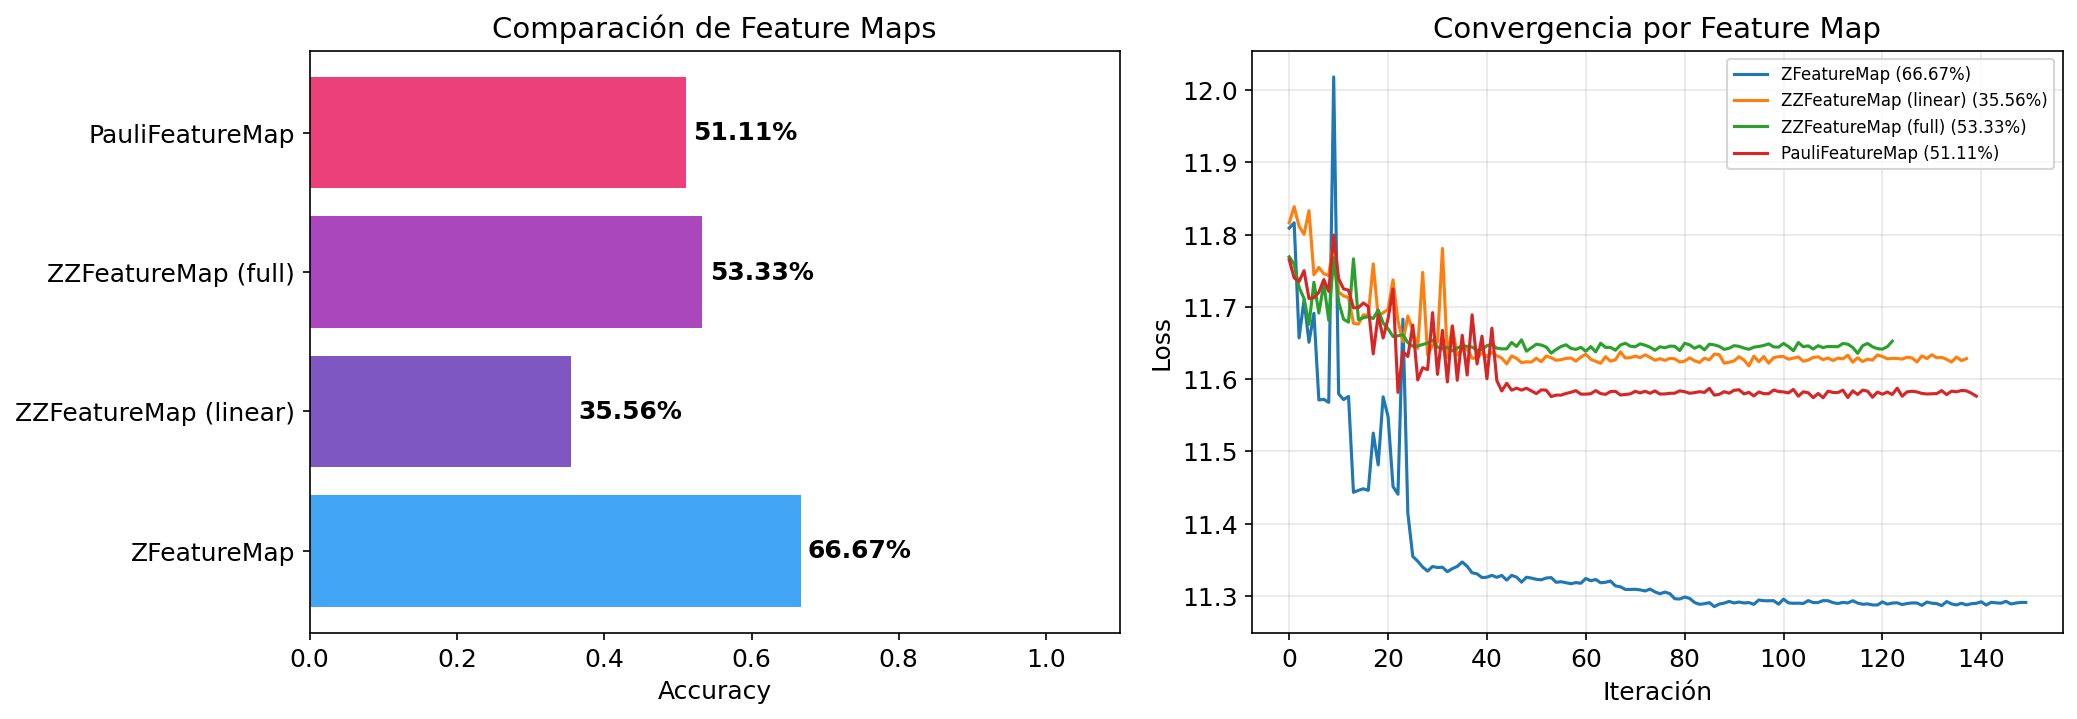
\includegraphics[width=0.92\textwidth]{figuras/exp1_feature_maps.png}
\caption{Izquierda: accuracy por feature map. Derecha: curvas de convergencia de la funci\'on de p\'erdida.}
\label{fig:featuremaps}
\end{figure*}

\subsection{Exp. 2: Profundidad del Ansatz}
Se vari\'o el n\'umero de repeticiones del ansatz RealAmplitudes (Tabla~\ref{tab:depth}). El accuracy mejor\'o con la profundidad, alcanzando 57.78\% con reps=5 (24 par\'ametros). No se observ\'o barren plateau en este rango.

\begin{table}[H]
\centering
\caption{Sensibilidad a la profundidad del ansatz}
\label{tab:depth}
\small
\begin{tabular}{cccc}
\toprule
\textbf{Reps} & \textbf{Par\'ams} & \textbf{Acc.} & \textbf{T (s)} \\
\midrule
1 & 8  & 0.333 & 44.5 \\
2 & 12 & 0.378 & 42.3 \\
3 & 16 & 0.489 & 40.7 \\
5 & 24 & 0.578 & 51.5 \\
\bottomrule
\end{tabular}
\end{table}

\begin{figure*}[t]
\centering
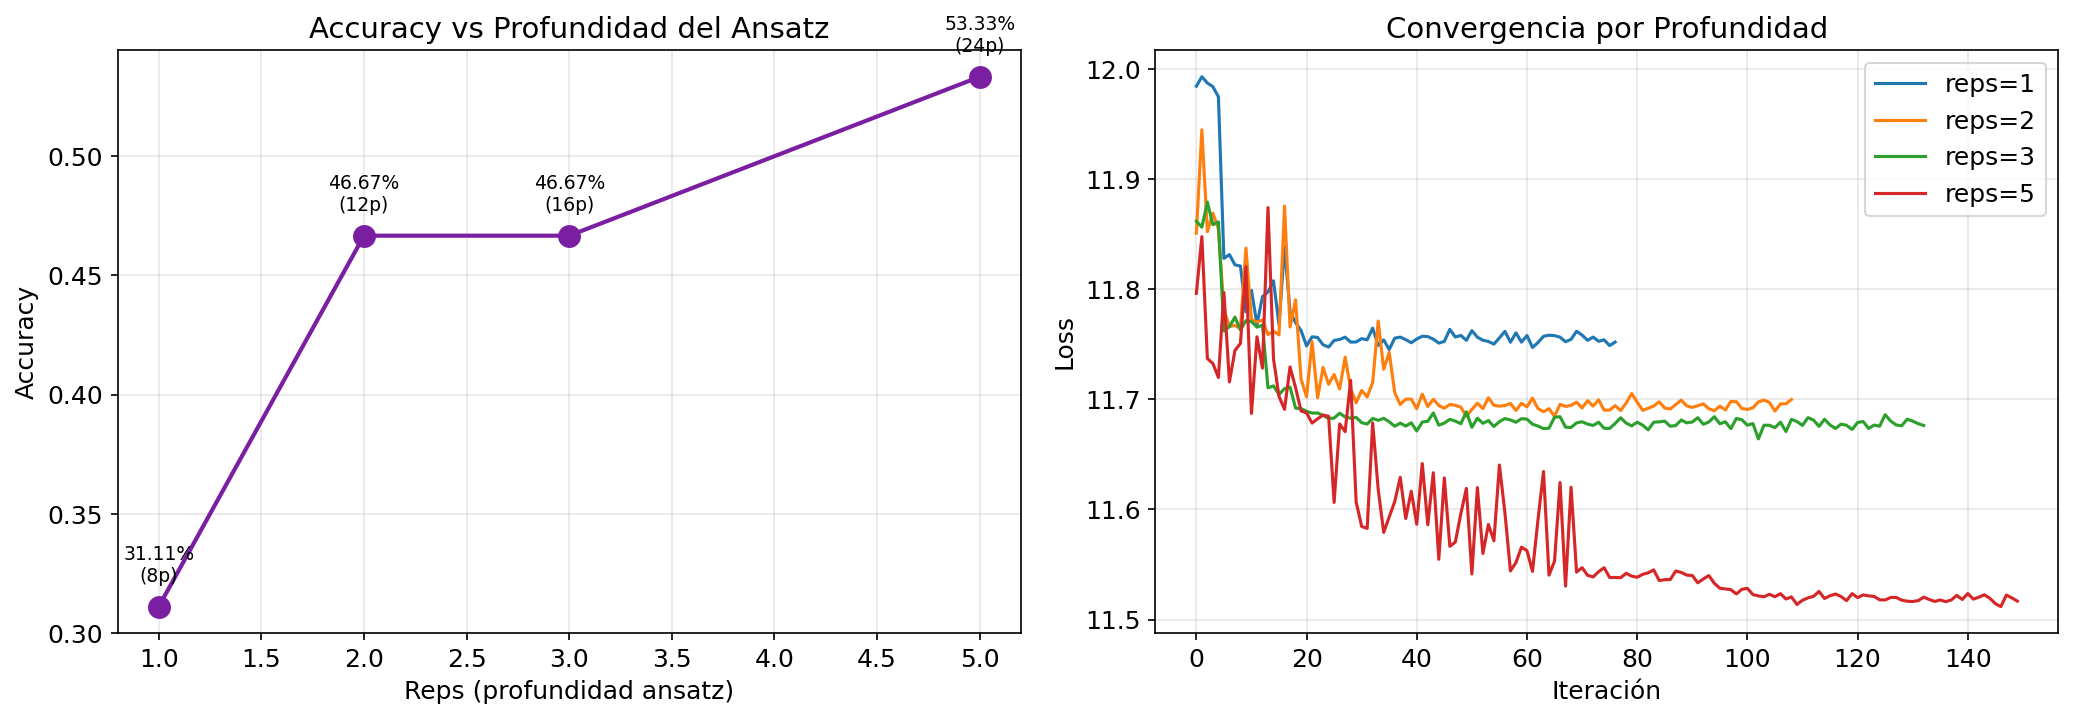
\includegraphics[width=0.92\textwidth]{figuras/exp2_profundidad.png}
\caption{Izquierda: accuracy vs n\'umero de repeticiones del ansatz. Derecha: convergencia por profundidad.}
\label{fig:depth}
\end{figure*}

\subsection{Exp. 3: Comparaci\'on de Optimizadores}
Se compararon tres optimizadores (Tabla~\ref{tab:optimizadores}). COBYLA obtuvo el mejor accuracy (62.22\%) con menor tiempo. L-BFGS-B fue el m\'as lento (204.1s) por el c\'alculo de gradientes.

\begin{table}[H]
\centering
\caption{Comparaci\'on de optimizadores}
\label{tab:optimizadores}
\small
\begin{tabular}{lccc}
\toprule
\textbf{Optim.} & \textbf{Acc.} & \textbf{Iter.} & \textbf{T (s)} \\
\midrule
COBYLA   & 0.622 & 177 & 43.9 \\
SPSA     & 0.556 & 150 & 149.1 \\
L-BFGS-B & 0.578 & 17  & 204.1 \\
\bottomrule
\end{tabular}
\end{table}

\begin{figure*}[t]
\centering
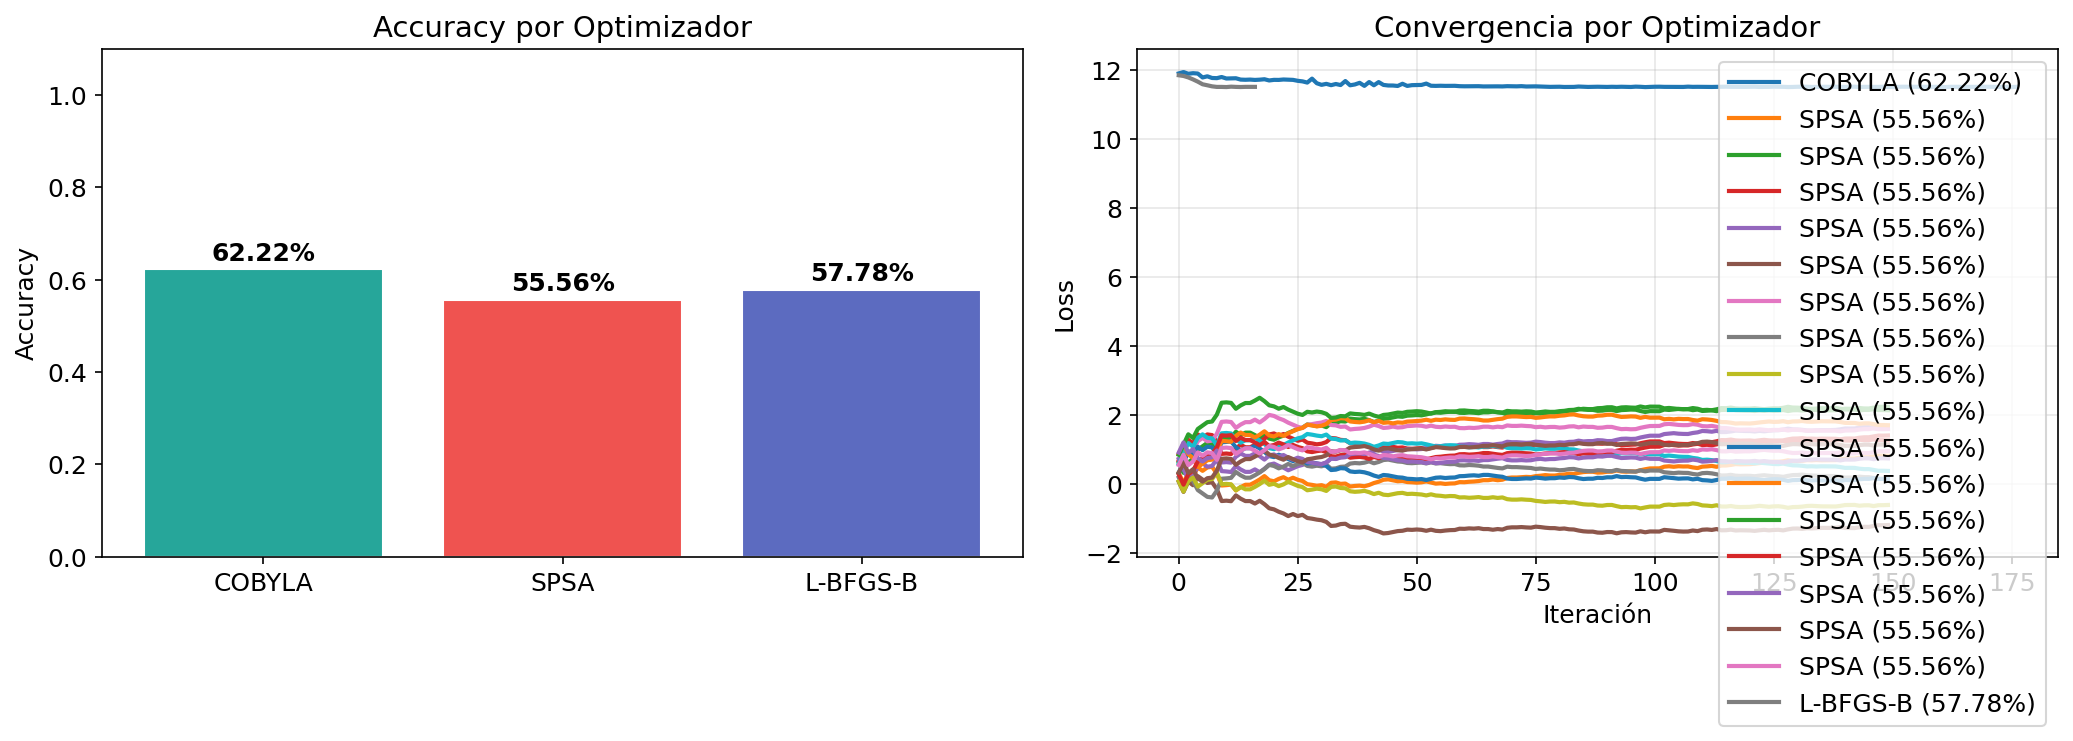
\includegraphics[width=0.92\textwidth]{figuras/exp3_optimizadores.png}
\caption{Izquierda: accuracy por optimizador. Derecha: curvas de convergencia de la funci\'on de p\'erdida.}
\label{fig:optimizadores}
\end{figure*}

\subsection{Kernel Cu\'antico vs Kernel RBF}
La Figura~\ref{fig:kernels} muestra los heatmaps de las matrices de kernel. El kernel cu\'antico exhibe una estructura m\'as dispersa y con mayor contraste, reflejando un mapeo diferente al espacio de caracter\'isticas.

\begin{figure}[H]
\centering
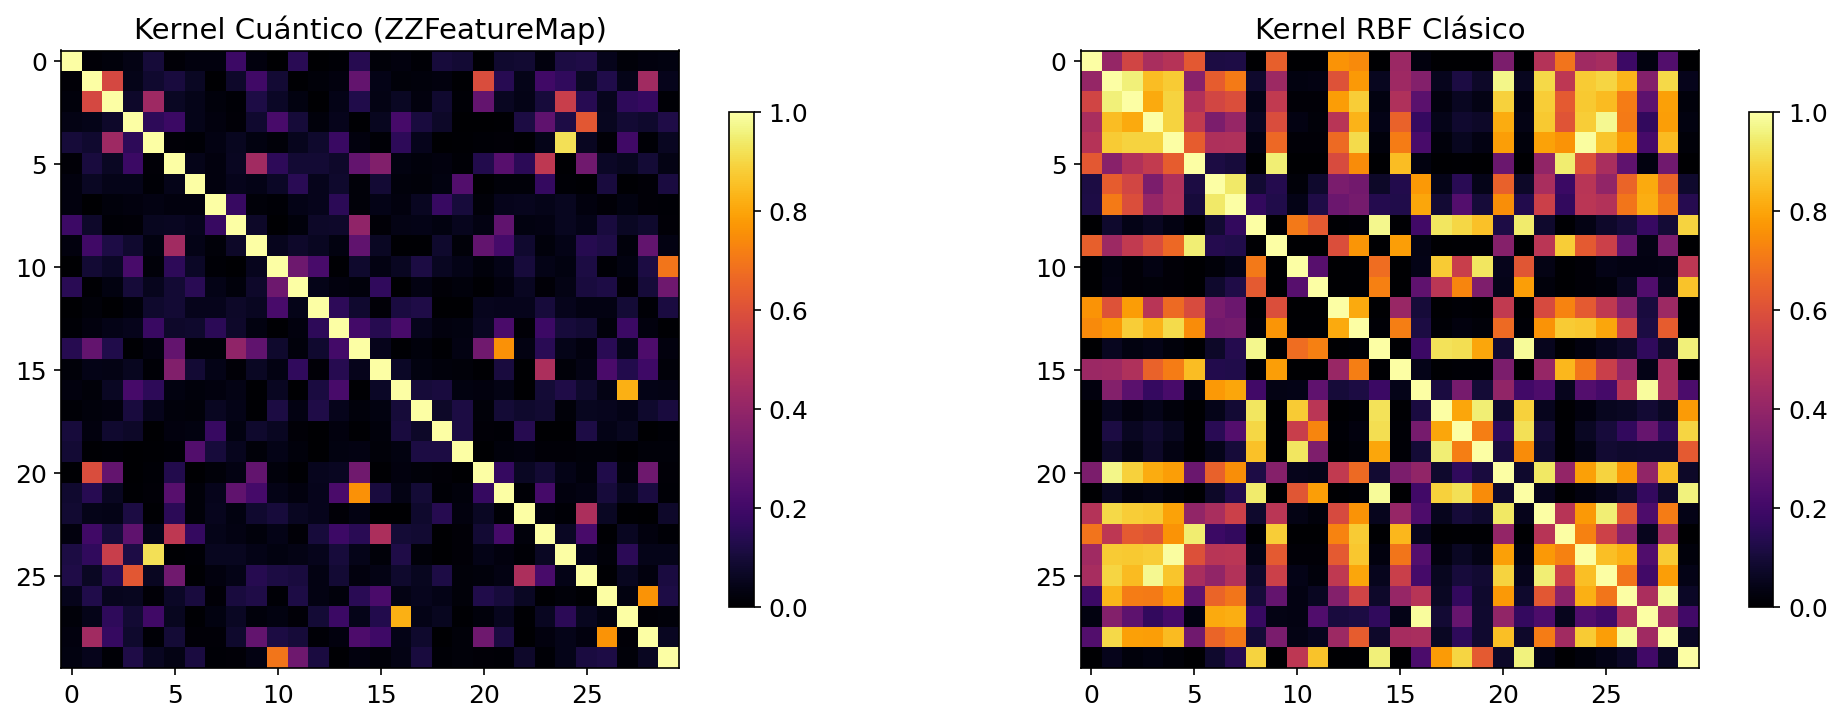
\includegraphics[width=\columnwidth]{figuras/kernels_heatmap.png}
\caption{Izq: kernel cu\'antico (ZZFeatureMap). Der: kernel RBF cl\'asico.}
\label{fig:kernels}
\end{figure}

\subsection{Varianza del VQC}
El VQC se ejecut\'o con 5 semillas distintas, obteniendo un accuracy promedio de $0.484 \pm 0.076$ (Figura~\ref{fig:varianza}). Esta varianza alta contrasta con el SVM-RBF ($0.960 \pm 0.039$ en validaci\'on cruzada 5-fold).

\begin{figure}[H]
\centering
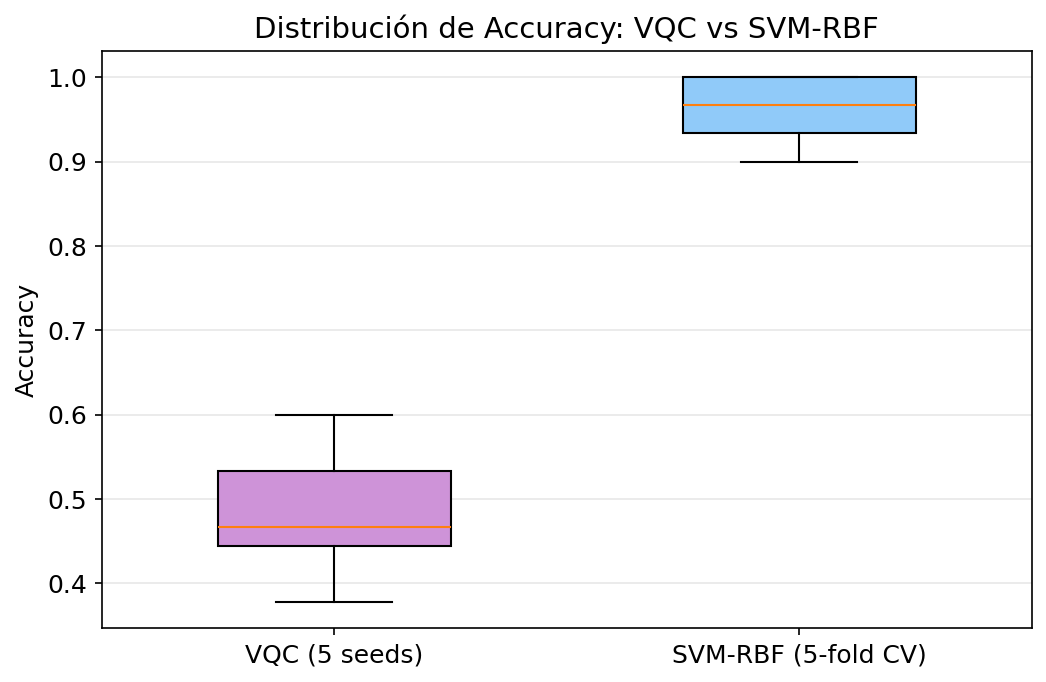
\includegraphics[width=\columnwidth]{figuras/boxplots_varianza.png}
\caption{Distribuci\'on de accuracy: VQC (5 semillas) vs SVM-RBF (5-fold CV).}
\label{fig:varianza}
\end{figure}

\subsection{MNIST Reducido}
En el dataset MNIST reducido (clases 0 vs 1), SVM-RBF alcanz\'o 100\% de accuracy mientras que VQC obtuvo 69.44\% (Figura~\ref{fig:mnist}). La tarea binaria es m\'as sencilla, pero el VQC a\'un no iguala al modelo cl\'asico.

\begin{figure*}[t]
\centering
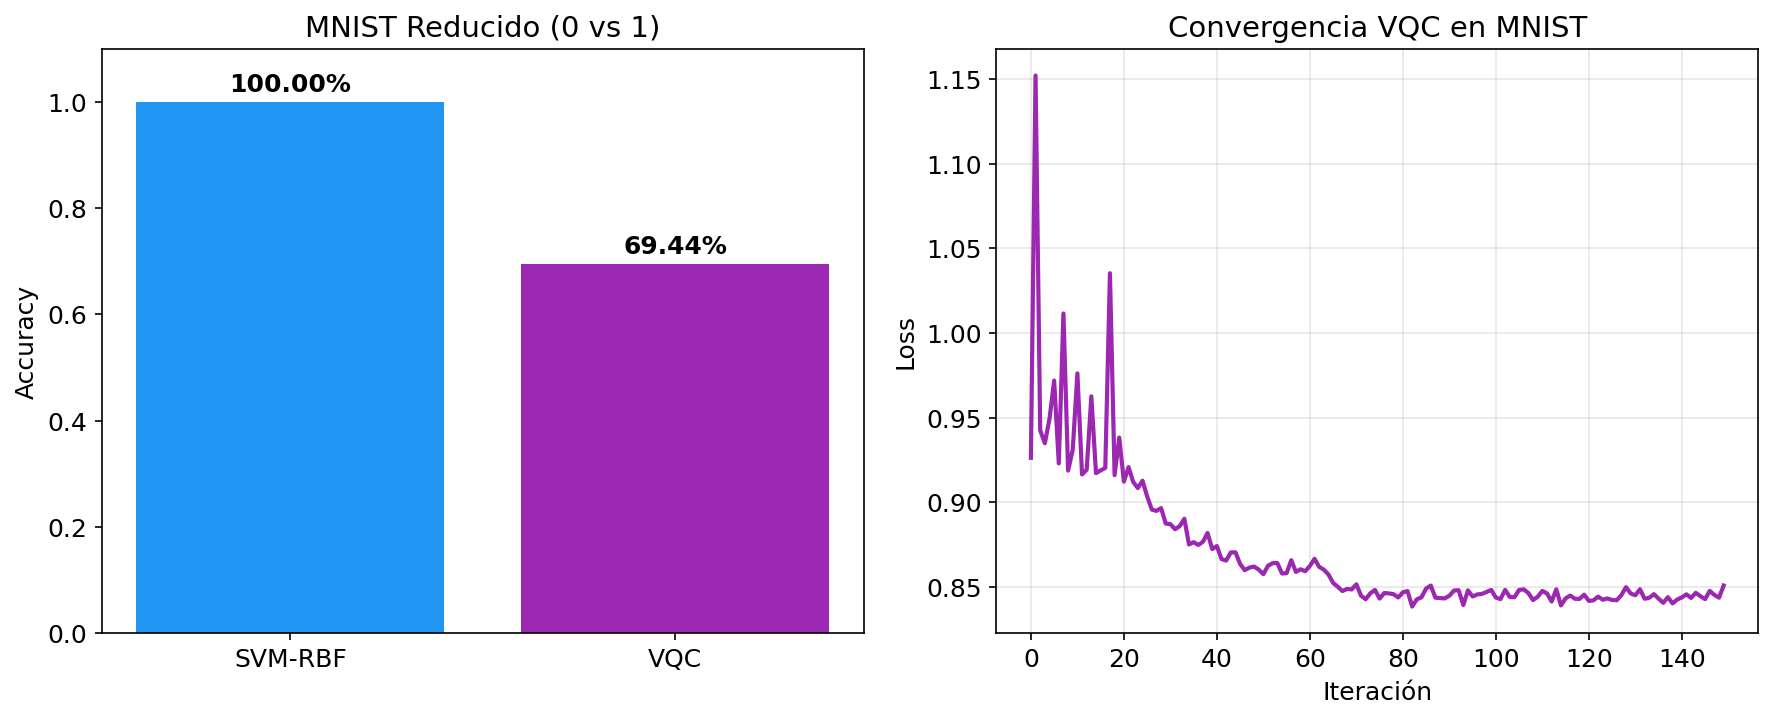
\includegraphics[width=0.92\textwidth]{figuras/exp_mnist.png}
\caption{Izquierda: accuracy SVM vs VQC en MNIST reducido. Derecha: convergencia del VQC.}
\label{fig:mnist}
\end{figure*}
